% Options for packages loaded elsewhere
\PassOptionsToPackage{unicode}{hyperref}
\PassOptionsToPackage{hyphens}{url}
\PassOptionsToPackage{dvipsnames,svgnames,x11names}{xcolor}
%
\documentclass[
  letterpaper,
  DIV=11,
  numbers=noendperiod]{scrartcl}

\usepackage{amsmath,amssymb}
\usepackage{iftex}
\ifPDFTeX
  \usepackage[T1]{fontenc}
  \usepackage[utf8]{inputenc}
  \usepackage{textcomp} % provide euro and other symbols
\else % if luatex or xetex
  \usepackage{unicode-math}
  \defaultfontfeatures{Scale=MatchLowercase}
  \defaultfontfeatures[\rmfamily]{Ligatures=TeX,Scale=1}
\fi
\usepackage{lmodern}
\ifPDFTeX\else  
    % xetex/luatex font selection
\fi
% Use upquote if available, for straight quotes in verbatim environments
\IfFileExists{upquote.sty}{\usepackage{upquote}}{}
\IfFileExists{microtype.sty}{% use microtype if available
  \usepackage[]{microtype}
  \UseMicrotypeSet[protrusion]{basicmath} % disable protrusion for tt fonts
}{}
\makeatletter
\@ifundefined{KOMAClassName}{% if non-KOMA class
  \IfFileExists{parskip.sty}{%
    \usepackage{parskip}
  }{% else
    \setlength{\parindent}{0pt}
    \setlength{\parskip}{6pt plus 2pt minus 1pt}}
}{% if KOMA class
  \KOMAoptions{parskip=half}}
\makeatother
\usepackage{xcolor}
\setlength{\emergencystretch}{3em} % prevent overfull lines
\setcounter{secnumdepth}{5}
% Make \paragraph and \subparagraph free-standing
\ifx\paragraph\undefined\else
  \let\oldparagraph\paragraph
  \renewcommand{\paragraph}[1]{\oldparagraph{#1}\mbox{}}
\fi
\ifx\subparagraph\undefined\else
  \let\oldsubparagraph\subparagraph
  \renewcommand{\subparagraph}[1]{\oldsubparagraph{#1}\mbox{}}
\fi


\providecommand{\tightlist}{%
  \setlength{\itemsep}{0pt}\setlength{\parskip}{0pt}}\usepackage{longtable,booktabs,array}
\usepackage{calc} % for calculating minipage widths
% Correct order of tables after \paragraph or \subparagraph
\usepackage{etoolbox}
\makeatletter
\patchcmd\longtable{\par}{\if@noskipsec\mbox{}\fi\par}{}{}
\makeatother
% Allow footnotes in longtable head/foot
\IfFileExists{footnotehyper.sty}{\usepackage{footnotehyper}}{\usepackage{footnote}}
\makesavenoteenv{longtable}
\usepackage{graphicx}
\makeatletter
\def\maxwidth{\ifdim\Gin@nat@width>\linewidth\linewidth\else\Gin@nat@width\fi}
\def\maxheight{\ifdim\Gin@nat@height>\textheight\textheight\else\Gin@nat@height\fi}
\makeatother
% Scale images if necessary, so that they will not overflow the page
% margins by default, and it is still possible to overwrite the defaults
% using explicit options in \includegraphics[width, height, ...]{}
\setkeys{Gin}{width=\maxwidth,height=\maxheight,keepaspectratio}
% Set default figure placement to htbp
\makeatletter
\def\fps@figure{htbp}
\makeatother

\KOMAoption{captions}{tableheading}
\makeatletter
\@ifpackageloaded{caption}{}{\usepackage{caption}}
\AtBeginDocument{%
\ifdefined\contentsname
  \renewcommand*\contentsname{Table of contents}
\else
  \newcommand\contentsname{Table of contents}
\fi
\ifdefined\listfigurename
  \renewcommand*\listfigurename{List of Figures}
\else
  \newcommand\listfigurename{List of Figures}
\fi
\ifdefined\listtablename
  \renewcommand*\listtablename{List of Tables}
\else
  \newcommand\listtablename{List of Tables}
\fi
\ifdefined\figurename
  \renewcommand*\figurename{Figure}
\else
  \newcommand\figurename{Figure}
\fi
\ifdefined\tablename
  \renewcommand*\tablename{Table}
\else
  \newcommand\tablename{Table}
\fi
}
\@ifpackageloaded{float}{}{\usepackage{float}}
\floatstyle{ruled}
\@ifundefined{c@chapter}{\newfloat{codelisting}{h}{lop}}{\newfloat{codelisting}{h}{lop}[chapter]}
\floatname{codelisting}{Listing}
\newcommand*\listoflistings{\listof{codelisting}{List of Listings}}
\makeatother
\makeatletter
\makeatother
\makeatletter
\@ifpackageloaded{caption}{}{\usepackage{caption}}
\@ifpackageloaded{subcaption}{}{\usepackage{subcaption}}
\makeatother
\ifLuaTeX
  \usepackage{selnolig}  % disable illegal ligatures
\fi
\usepackage{bookmark}

\IfFileExists{xurl.sty}{\usepackage{xurl}}{} % add URL line breaks if available
\urlstyle{same} % disable monospaced font for URLs
\hypersetup{
  pdftitle={R을 이용한 데이터 전처리와 시각화 기초 코스},
  colorlinks=true,
  linkcolor={blue},
  filecolor={Maroon},
  citecolor={Blue},
  urlcolor={Blue},
  pdfcreator={LaTeX via pandoc}}

\title{R을 이용한 데이터 전처리와 시각화 기초 코스}
\author{}
\date{}

\begin{document}
\maketitle

\renewcommand*\contentsname{Table of contents}
{
\hypersetup{linkcolor=}
\setcounter{tocdepth}{3}
\tableofcontents
}

\includegraphics{typst2_files/mediabag/1200px-R_logo.svg.png}

\section{1 Introduction}\label{introduction}

이 수업은 코딩을 전혀 모르는 사람들을 대상으로 숫자로 된 데이터를 적절히
칼질하여 요리할 수 있도록 하는 것을 목적으로 만들었습니다.

반복적으로 정형화된 데이터를 처리하고 그래프를 그리는 연구원들은
최종적으로는 자신의 결과물을 알기 쉽게 표현하는 것입니다.

이를 위해 tidyverse 패키지 하나만으로 얼마나 쉽게 데이터를 다룰 수
있는지 R의 장점이 무엇인지 알 수 있는 시간이 될 것입니다.

\textbf{R 언어 간단 소개}

두명의 뉴질랜드 통계학자가 만듦 : 로버트 젠틀맨(Robert Gentleman)과 로스
이하카(Ross Ihaka)

해들리 위컴에 의해 빅데이터 툴로 발전함 (대표적 : ggplot, tidyverse)


\includegraphics{typst2_files/mediabag/9.28-1.png}

\textbf{언어의 특징}

1부터 시작 (다른 언어들은 0부터 시작)

\textbf{패키지 설치, 불러오기}

\begin{itemize}
\item
  install.packages(``패키지이름'')
\item
  library(패키지이름)
\end{itemize}

\subsection{프로그램 구분}\label{uxd504uxb85cuxadf8uxb7a8-uxad6cuxbd84}

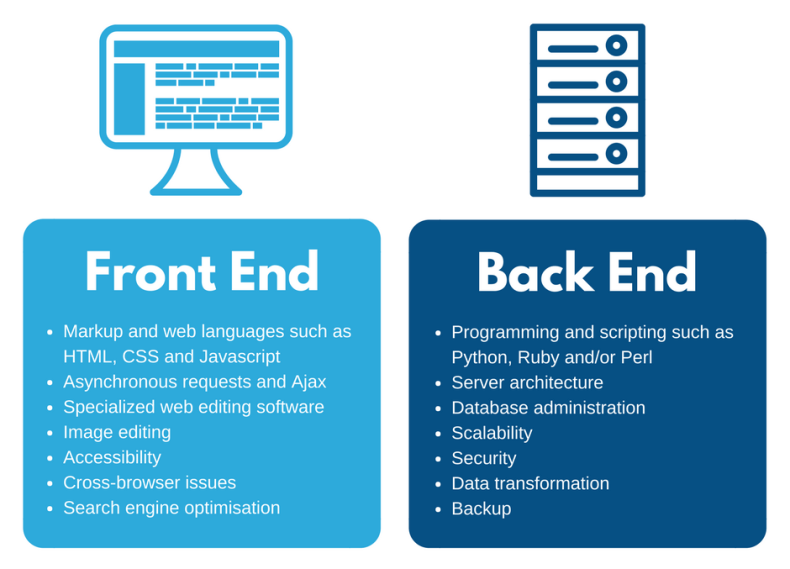
\includegraphics{typst2_files/mediabag/img.png}

Back end를 담당하는 데이터 전처리 및 시각화는 tidyverse 패키지를
이용하여 진행하고 필요할 경우, 추가 패키지를 이용할 것입니다.

실전에서 바로 쓸 수 있도록 기본 예제 데이터를 이용하여 학습하고 각자
자신의 자주 사용하는 데이터를 이용하여 반복 적으로 하던 일을 코딩을 통해
줄이고 더 창의적인 일에 시간을 쓸 수 있도록 8주 과정으로 만들었습니다.
(주1회 2시간, 총 16시간)

이 과정을 공부하고 나면 현업에서 이미지가 아닌 숫자로 된 데이터를 다양한
전처리, 시각화, 머신러닝을 통한 예측을 할 수 있게 될 것이며, 빅데이터
분석기사 필기 시험을 통과할 수 있을 수준이 될 것입니다.

\section{2 강의순서}\label{uxac15uxc758uxc21cuxc11c}

\begin{enumerate}
\def\labelenumi{\arabic{enumi}.}
\item
  R 설치, 기본문법 (1주차)

  \url{https://dplyr.tidyverse.org/articles/dplyr.html}
\item
  데이터 전처리 dplyr (2주차)

  \url{https://m-clark.github.io/data-processing-and-visualization/intro.html}
\item
  데이터 전처리 문제 풀이 (3주차)

  \url{https://m-clark.github.io/data-processing-and-visualization/intro.html}
\item
  데이터 시각화 ggplot (4주차)

  \url{https://r-graph-gallery.com/}
\item
  다양한 데이터 시각화 연습 (5주차)

  2d, 3d 이미지화

  \begin{itemize}
  \tightlist
  \item
    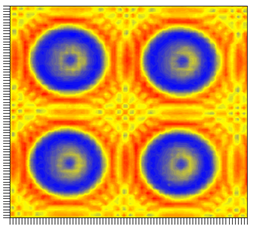
\includegraphics{images/logo1.png}
  \end{itemize}
\item
  다양한 데이터 시각화 연습2 (6주차)

  \begin{itemize}
  \item
    html로 문서 만들기

    \url{https://waterfirst.github.io/LENS_EXPERIMENT/}
  \end{itemize}
\item
  머신러닝 기본문법 및 예제 (7주차)

  \begin{itemize}
  \tightlist
  \item
    회귀분석
  \end{itemize}
\item
  머신러닝 기본문법 및 예제 (8주차)

  \begin{itemize}
  \tightlist
  \item
    분류
  \end{itemize}
\end{enumerate}



\end{document}
